\documentclass[12pt,letterpaper]{article}

%% ── Packages ────────────────────────────────────────────────────────────────
\usepackage[margin=1in]{geometry}
\usepackage{setspace}
\usepackage[round,authoryear]{natbib}
\usepackage{booktabs}
\usepackage{threeparttable}
\usepackage{makecell}

%% ── Redefine tablenotes to accept free-form text (no \item required) ─────────
\makeatletter
\renewenvironment{tablenotes}{%
  \par\vspace{2pt}%
  \begin{minipage}{\linewidth}%
  \singlespacing%
}{%
  \end{minipage}%
}
\makeatother
\usepackage{graphicx}
\usepackage{amsmath,amssymb}
\usepackage{microtype}
\usepackage{caption}
\usepackage{subcaption}
\usepackage{pifont}
\usepackage{xcolor}
\usepackage[hidelinks,
            pdfauthor={Carlos C\'esar Ch\'avez Padilla},
            pdftitle={Monetary Policy Transmission in Peru}]{hyperref}

%% ── Custom symbols ──────────────────────────────────────────────────────────
\newcommand{\cmark}{\ding{51}}
\newcommand{\xmark}{\ding{55}}
\newcommand{\warnmark}{$\triangle$}

%% ── Double spacing ──────────────────────────────────────────────────────────
\doublespacing

%% ── Caption style ───────────────────────────────────────────────────────────
\captionsetup{font=small,labelfont=bf,skip=4pt}

%% ── Convenience environment for floated tables ──────────────────────────────
\newenvironment{mytable}[2]{%
  \begin{table}[htbp]
  \centering
  \caption{#1}
  \label{#2}
  \begin{threeparttable}
}{%
  \end{threeparttable}
  \end{table}
}

%% ── Missing from standard natbib ────────────────────────────────────────────
\newcommand{\sims}{Sims}

\begin{document}

% ─────────────────────────────────────────────────────────────────────────────
\begin{titlepage}
\vspace*{2cm}
{\singlespacing
\begin{center}
  {\LARGE\bfseries Monetary Policy Transmission in Peru:\\[6pt]
   A Systematic Comparison of Identification Strategies}

  \bigskip\bigskip

  {\large Carlos C\'{e}sar Ch\'{a}vez Padilla}\\[4pt]
  {\normalsize Center for the Economics of Human Development\\
   University of Chicago}

  \bigskip

  {\normalsize March 2026}

  \bigskip\bigskip

  \begin{abstract}
    \noindent
    We estimate the effects of monetary policy on GDP and poverty in Peru
    using quarterly data from 2004Q2 to 2025Q3 ($T=85$). We systematically
    compare seven identification strategies---recursive (Cholesky), sign
    restrictions, narrative sign restrictions, local projections, two
    Proxy-SVAR approaches using interbank rate surprises and AI-classified
    BCRP communication tone (325 \textit{Notas Informativas}, 2001--2026),
    and a GDP--poverty reduced-form regression---and find that only recursive
    identification produces interpretable estimates. The Cholesky VAR(1)
    yields a peak GDP response of $-0.195$\,pp per 100\,bp rate hike
    (90\% bootstrap CI: $[-0.698,\,+0.271]$), consistent with the Peru SVAR
    literature ($-0.25$ to $-0.30$\,pp). Modern identification methods fail
    because Peru's interbank rate is administered, no rate-futures market
    exists for policy surprise extraction, and the monetary record since 2003
    provides too few sharp episodes for narrative restrictions.
    Our most robust result is a GDP--poverty elasticity of $\hat\beta=-0.656$
    ($t=-5.69$, $R^2=0.67$, $N=18$), estimated from ENAHO annual data
    2005--2024 and stable across sub-periods. Chaining the two elasticities
    implies a 100\,bp hike may raise poverty by approximately $+0.13$\,pp,
    though this inherits the large uncertainty of the rate--GDP link.
    The paper explains why the Peru SVAR literature relies on recursive
    identification and cautions against applying Proxy-SVAR and narrative
    methods---developed for the US and Euro Area---to emerging markets with
    administered policy rates.
  \end{abstract}

  \medskip
  {\footnotesize
  \textit{JEL codes:} E52, E32, I32, C32.\\
  \textit{Keywords:} monetary policy transmission, SVAR, local projections,
  narrative identification, Proxy-SVAR, poverty, Peru.}
\end{center}
}
\end{titlepage}

% ─────────────────────────────────────────────────────────────────────────────
\section{Introduction}
\label{sec:intro}

Understanding how monetary policy transmits to real activity is a central
question in macroeconomics. The global literature has developed an expanding
identification toolkit: recursive (Cholesky) ordering, sign restrictions
\citep{uhlig2005}, narrative restrictions \citep{antolin2018}, and
external-instrument Proxy-SVARs \citep{stock2018,gertler2015,montiellolea2021}.
These methods have been applied extensively to the United States and Euro Area,
and increasingly to advanced economies such as Australia. Their applicability
to small open emerging-market economies (EMEs) with institutional features
that differ markedly from the US---administered policy rates, no OIS market,
limited monetary history---has received far less systematic attention.

Peru offers a particularly instructive case. The Banco Central de Reserva del
Per\'{u} (BCRP) has operated a credible inflation-targeting framework since
2002, with a target of $2\%\pm1$\,pp. Yet Peru's monetary implementation
differs fundamentally from the US Federal Reserve: the interbank overnight
rate is \emph{administered}---the BCRP ensures the interbank rate equals
the reference rate by construction, leaving no market-determined component
from which to extract policy surprises. This single institutional feature,
combined with the absence of rate-futures markets and a relatively
uneventful monetary history, renders the modern identification toolkit mostly
inapplicable.

The existing Peru-specific literature---\citet{perezrojo2024},
\citet{castillo2011}, and \citet{portilla2022}---uniformly relies on
recursive identification without documenting why more modern alternatives
fail. This paper fills that gap with four contributions:

\begin{enumerate}
  \item \textbf{First systematic comparison} of seven identification
    strategies for monetary policy in Peru within a single unified dataset
    ($T=85$, 2004Q2--2025Q3; see Table~\ref{tab:master}).

  \item \textbf{First Proxy-SVAR with BCRP communication analysis:} we
    classify 325 \textit{Notas Informativas del Programa Monetario}
    (2001--2026) using both a hawkish/dovish dictionary and a large
    language model (Claude Haiku, $-100$ to $+100$ scale), yielding the
    most comprehensive BCRP tone dataset to date (Table~\ref{tab:tone_class}).

  \item \textbf{A well-identified GDP--poverty elasticity}
    ($\hat\beta=-0.656$, $p<0.001$, $N=18$; Table~\ref{tab:poverty_ols})
    that chains monetary policy effects to poverty outcomes, stable across
    sub-periods (Table~\ref{tab:subperiod}).

  \item \textbf{An explanation of why modern identification fails} in Peru's
    institutional environment, contributing to the emerging literature on
    monetary policy transmission in EMEs \citep{ha2025}.
\end{enumerate}

The Cholesky benchmark (Figure~\ref{fig:cholesky_irfs}) yields a peak GDP
response of $-0.195$\,pp per 100\,bp consistent with published Peru
estimates. Sign restrictions produce an identified set too wide for
inference. Narrative restrictions are blocked by a fundamental
COVID-dummy--narrative tension. Proxy-SVAR with the interbank rate fails
relevance ($F=4.73$; Table~\ref{tab:proxy_ib}), and Proxy-SVAR with tone
passes relevance only when the instrument retains anticipated policy (violating
exogeneity; Table~\ref{tab:tone_iv}).

Section~\ref{sec:background} describes Peru's monetary framework.
Section~\ref{sec:data} presents the data. Section~\ref{sec:framework}
develops the econometric framework. Section~\ref{sec:results} reports
results. Section~\ref{sec:comparison} presents the master comparison.
Section~\ref{sec:discussion} discusses implications.
Section~\ref{sec:conclusion} concludes.

% ─────────────────────────────────────────────────────────────────────────────
\section{Institutional Background}
\label{sec:background}

\subsection{BCRP Monetary Policy Framework}

The BCRP adopted inflation targeting in 2002, with a target band of
$2\%\pm1$\,pp. The reference rate is announced monthly on a pre-set
calendar. Unlike the Federal Reserve, the BCRP keeps the interbank
overnight rate equal to the reference rate through active liquidity
provision or absorption, making it administered by construction.

Additional distinguishing features include: (i) active foreign exchange
intervention in a managed float; (ii) partial dollarization, with significant
deposits and credit in both Peruvian soles (PEN) and US dollars; and (iii) the
absence of any OIS or rate-futures market for PEN, precluding high-frequency
extraction of market rate expectations.

\subsection{Why Peru Differs from the US and Euro Area}

Three features make modern identification strategies particularly difficult.

\paragraph{Administered interbank rate.} The interbank rate equals the
reference rate by BCRP design, leaving no ``surprise'' component in the sense
of \citet{gertler2015}. The interbank ``surprise'' used as a Proxy-SVAR
instrument is mechanically collinear with the reference rate change already
in the VAR (Section~\ref{sec:proxy_ib}).

\paragraph{No rate expectations market.} Without OIS or futures contracts
on PEN rates, it is impossible to separate the expected from the unexpected
component of a rate decision, as is standard in the US literature
\citep{mirandaagrippino2021}.

\paragraph{Limited sharp monetary episodes.} Since 2002, BCRP changes have
been small and gradual, with only two exceptions: the emergency COVID cuts of
2020 (2.25\% to 0.25\%) and the 2021--2022 hiking cycle (0.25\% to 7.75\%).
As \citet{read2023} demonstrate, even the US narrative identification
literature struggles with fewer than a handful of clear episodes; two
episodes are insufficient for Peru.

\subsection{BCRP Reference Rate History}

Figure~\ref{fig:bcrp_rate} shows the BCRP reference rate from 2003 to
2025Q3, with key episodes annotated: the GFC cutting cycle (2008--2009,
from 6.5\% to 1.25\%), the 2010--2011 hiking cycle (to 4.25\%), gradual
cuts in 2014--2015, the COVID emergency cuts to 0.25\% in 2020, the
aggressive 2021--2022 hiking cycle to 7.75\%, and subsequent easing to
4.25\% by end-2025.

\begin{figure}[htbp]
  \centering
  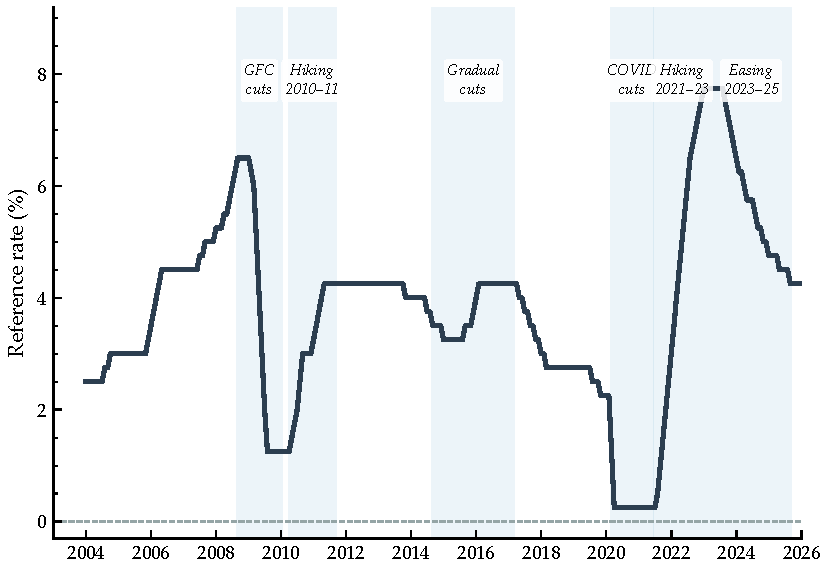
\includegraphics[width=\textwidth]{figures/fig1_bcrp_rate_path}
  \caption{BCRP Reference Rate, 2003--2025. Key episodes: GFC cuts
    (2008--2009), 2010--2011 hiking cycle, COVID emergency cuts to
    0.25\% (2020), aggressive hiking to 7.75\% (2021--2022), and
    gradual easing (2023--2025). Source: BCRP series PD04722MM.}
  \label{fig:bcrp_rate}
\end{figure}

% ─────────────────────────────────────────────────────────────────────────────
\section{Data}
\label{sec:data}

\subsection{Macroeconomic Variables}

The VAR uses five quarterly series from the BCRP data portal: terms of
trade (PN38923BM), real GDP quarter-on-quarter growth (PN01731AM,
summed from monthly seasonally adjusted index), CPI quarter-on-quarter
change (PN01271PM), PEN/USD exchange rate change (PN01246PM), and BCRP
reference rate change (PD04722MM). The sample runs from 2004Q2 to 2025Q3
($T=85$). Summary statistics are in Table~\ref{tab:sumstats}; all series
are stationary by ADF tests ($p<0.001$ for each).

COVID treatment follows the Frisch-Waugh-Lovell (FWL) principle: indicator
variables for 2020Q1 and 2020Q2 are partialled out of all series before
estimation. This is preferred to a contemporaneous dummy in the VAR because
a dummy in $Y_t$ but not the lags creates inconsistency in VAR($p\geq2$)
systems by contaminating lagged regressors.

\begin{mytable}{Summary Statistics, 2004Q2--2025Q3}{tab:sumstats}
  
\begin{tabular}{lrrrrcc}
\toprule
Variable & Mean & SD & Min & Max & ADF stat & ADF $p$ \\
\midrule
    GDP (qoq, pp) & 0.013 & 2.810 & -10.890 & 4.851 & -4.80 & 0.000 \\
    CPI (qoq, pp) & 0.527 & 0.574 & -0.680 & 2.510 & -5.66 & 0.000 \\
    FX (qoq, $\%\Delta$) & 0.085 & 2.104 & -6.502 & 5.900 & -6.50 & 0.000 \\
    Rate ($\Delta$ pp) & 0.009 & 0.503 & -1.250 & 1.250 & -5.90 & 0.000 \\
    ToT (qoq, pp) & 0.170 & 4.050 & -16.010 & 9.220 & -7.51 & 0.000 \\
\bottomrule
\end{tabular}
\begin{tablenotes}
\small Sample: 2004Q2--2025Q3 ($T=85$). ADF with intercept; all series stationary.
COVID FWL: 2020Q1--Q2 partialled out in estimation.
\end{tablenotes}

\end{mytable}

\subsection{BCRP Communications Corpus}

We construct a dataset of 325 \textit{Notas Informativas del Programa
Monetario}---the official monthly communications explaining each rate
decision---covering 2001 to 2026. Documents were downloaded from the BCRP
website and the Wayback Machine; text was extracted with \texttt{pdfplumber}.

Each note is classified by tone using two methods: (a) a dictionary-based
approach using a hawkish/dovish lexicon adapted from \citet{lahura2020},
producing scores in $[-1,+1]$; and (b) an LLM-based approach using Claude
Haiku, prompted to score each note on $[-100,+100]$. Table~\ref{tab:tone_class}
presents classification statistics. The correlation between dictionary and
LLM scores is $0.373$, indicating moderate agreement. Both methods
correctly flag 2009 as dovish and 2022 as hawkish. Figure~\ref{fig:tone}
shows the tone series over time.

\begin{mytable}{BCRP Communication Tone: Summary Statistics}{tab:tone_class}
  
\begin{tabular}{lcc}
\toprule
Statistic & Dictionary & LLM (Claude Haiku) \\
\midrule
    Corpus size (notes) & \multicolumn{2}{c}{324} \\
    Date range & \multicolumn{2}{c}{2001--2026} \\
    Mean score & -0.059 & -7.8 \\
    SD & 0.510 & 40.2 \\
    Min & -1.0 & -85 \\
    Max & 1.0 & 75 \\
    Correlation (dict vs LLM) & \multicolumn{2}{c}{0.380} \\
\bottomrule
\end{tabular}
\begin{tablenotes}
\small Dictionary: hawkish/dovish lexicon adapted from Lahura \& Vega (2020 CEMLA).
LLM: Claude Haiku (\texttt{claude-haiku-4-5-20251001}), prompt scored each
Nota Informativa on $[-100, +100]$ with chain-of-thought rationale.
\end{tablenotes}

\end{mytable}

\begin{mytable}{BCRP Communication Tone by Year, 2001--2026}{tab:tone}
  
\scalebox{0.78}{\begin{tabular}{lrcccc}
\toprule
Year & $N$ & Dict. mean & (SD) & LLM mean & (SD) \\
\midrule
    2001 & 12 & 0.00 & (0.60) & -50.0 & (16.2) \\
    2002 & 13 & 0.46 & (0.53) & -10.4 & (34.2) \\
    2003 & 10 & 0.17 & (0.81) & -21.0 & (25.3) \\
    2004 & 12 & 0.08 & (0.36) & 9.2 & (22.7) \\
    2005 & 12 & -0.27 & (0.46) & -5.8 & (14.7) \\
    2006 & 13 & 0.47 & (0.32) & 15.8 & (21.1) \\
    2007 & 14 & 0.47 & (0.34) & 31.4 & (29.6) \\
    2008 & 17 & 0.22 & (0.51) & 27.6 & (53.2) \\
    2009 & 13 & -0.53 & (0.53) & -57.3 & (32.2) \\
    2010 & 15 & 0.32 & (0.57) & 12.0 & (40.5) \\
    2011 & 12 & -0.05 & (0.84) & 15.0 & (41.3) \\
    2012 & 12 & -0.26 & (0.36) & -3.8 & (9.3) \\
    2013 & 13 & -0.36 & (0.36) & -9.6 & (21.0) \\
    2014 & 12 & -0.52 & (0.14) & -25.8 & (16.2) \\
    2015 & 15 & -0.53 & (0.24) & -13.0 & (29.8) \\
    2016 & 15 & -0.45 & (0.26) & 0.3 & (28.4) \\
    2017 & 12 & -0.17 & (0.19) & -22.9 & (17.9) \\
    2018 & 13 & 0.03 & (0.17) & -26.2 & (19.2) \\
    2019 & 13 & 0.20 & (0.30) & -30.4 & (17.1) \\
    2020 & 14 & -0.30 & (0.37) & -65.0 & (24.5) \\
    2021 & 12 & -0.31 & (0.34) & -22.5 & (42.0) \\
    2022 & 12 & 0.06 & (0.25) & 74.2 & (2.9) \\
    2023 & 12 & -0.05 & (0.10) & 9.2 & (36.0) \\
    2024 & 12 & -0.23 & (0.17) & -26.2 & (25.8) \\
    2025 & 12 & -0.17 & (0.38) & -15.0 & (19.9) \\
\midrule
    Overall & 322 &
    -0.069 & (0.380) &
    -8.4 & (25.6) \\
\bottomrule
\end{tabular}}
\begin{tablenotes}
\small LLM: Claude Haiku, score $-100$ (dovish) to $+100$ (hawkish).
Dict.: dictionary method (Lahura \& Vega 2020 adaptation).
\end{tablenotes}

\end{mytable}

\begin{figure}[htbp]
  \centering
  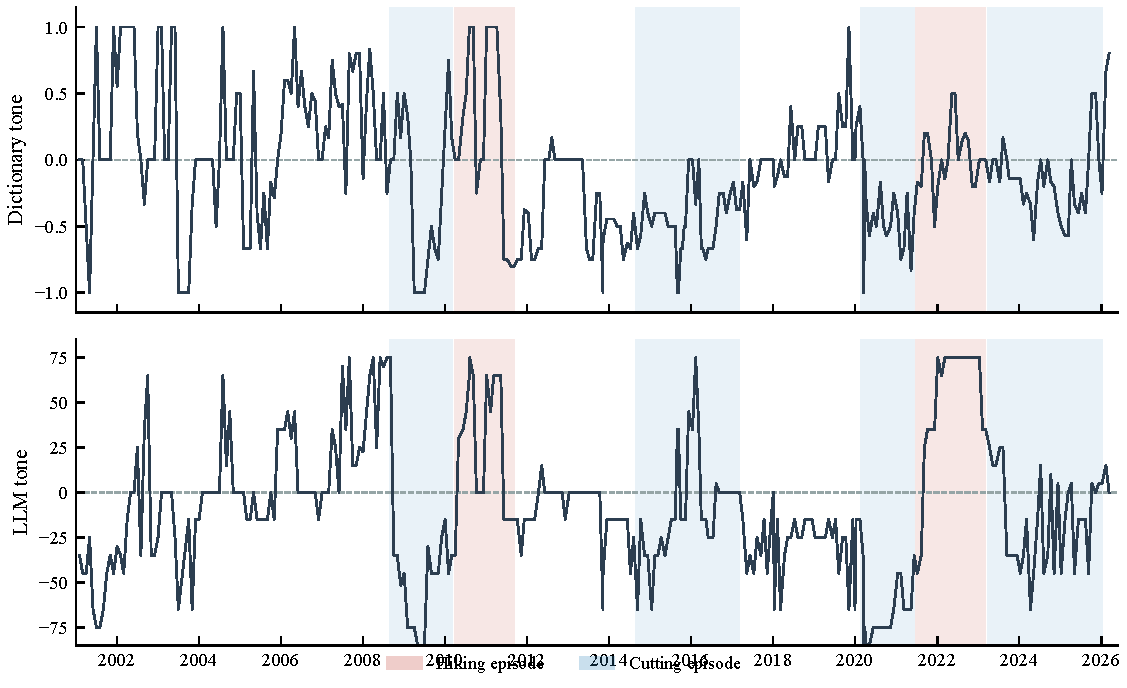
\includegraphics[width=\textwidth]{figures/fig6_bcrp_tone_series}
  \caption{BCRP Communication Tone, 2001--2026. Bars: dictionary score
    (left axis). Line: LLM score (right axis). Both flag 2009 (GFC
    emergency cuts) as strongly dovish and 2022 (hiking cycle) as hawkish.
    Dictionary--LLM correlation: $r=0.373$.}
  \label{fig:tone}
\end{figure}

\subsection{Poverty Data}

The poverty measure is the official annual monetary poverty headcount ratio
from INEI/ENAHO household surveys, 2005--2024. COVID years 2020--2021 are
excluded due to lockdown disruptions and INEI methodology changes. The
regression sample contains $N=18$ annual observations. Table~\ref{tab:poverty}
lists the full dataset.

\begin{mytable}{Annual GDP Growth and Poverty Data, 2005--2024}{tab:poverty}
  
\begin{tabular}{lrr}
\toprule
Year & GDP growth (\%) & $\Delta$Poverty (pp) \\
\midrule
    2005 & 6.282 & $-2.7$ \\
    2006 & 7.555 & $-5.0$ \\
    2007 & 8.470 & $-6.3$ \\
    2008 & 9.185 & $-5.0$ \\
    2009 & 1.123 & $-3.4$ \\
    2010 & 8.283 & $-4.5$ \\
    2011 & 6.380 & $-3.5$ \\
    2012 & 6.145 & $-2.3$ \\
    2013 & 5.827 & $-1.7$ \\
    2014 & 2.453 & $-0.4$ \\
    2015 & 3.223 & $-1.7$ \\
    2016 & 3.975 & $-1.1$ \\
    2017 & 2.515 & $\phantom{-}0.0$ \\
    2018 & 3.957 & $-1.6$ \\
    2019 & 2.250 & $-0.6$ \\
    2022 & 2.857 & $1.5$ \\
    2023 & $-0.345$ & $1.5$ \\
    2024 & 3.473 & $-2.1$ \\
\bottomrule
\end{tabular}
\begin{tablenotes}
\small GDP: BCRP national accounts, annual average YoY real growth.
Poverty: INEI-ENAHO monetary poverty rate. 2020--2021 excluded (COVID).
2022 and 2023 reflect K-shaped recovery and post-pandemic return to normal.
\end{tablenotes}

\end{mytable}

% ─────────────────────────────────────────────────────────────────────────────
\section{Econometric Framework}
\label{sec:framework}

\subsection{Reduced-Form VAR}

The baseline model is a VAR($p$):
\begin{equation}
  Y_t = c + A_1 Y_{t-1} + \cdots + A_p Y_{t-p} + u_t, \quad
  u_t \sim \mathcal{N}(0,\Sigma),
  \label{eq:var}
\end{equation}
where $Y_t = (\mathrm{tot}_t,\, \mathrm{gdp}_t,\, \mathrm{cpi}_t,\,
\mathrm{fx}_t,\, \mathrm{rate}_t)'$. COVID quarters are handled via FWL.
AIC and BIC both select $p=1$.

\subsection{Identification Strategies}

\paragraph{Strategy 1 (Cholesky).}
We impose a lower-triangular Cholesky decomposition $\hat\Sigma=PP'$ and
identify the monetary policy shock as the innovation to the rate equation
after conditioning on same-quarter innovations to ToT, GDP, CPI, and FX.
The ordering ToT $\to$ GDP $\to$ CPI $\to$ FX $\to$ Rate embeds the
assumption that the BCRP does not react within-quarter to real activity
or inflation, consistent with Peru's monthly-calendar announcement system.

\paragraph{Strategy 2 (Sign Restrictions).}
Following \citet{uhlig2005}, we identify the monetary shock $\varepsilon^{mp}_t$
by requiring
\begin{equation}
  \frac{\partial\,\mathrm{rate}_{t+h}}{\partial\,\varepsilon^{mp}_t}>0
  \;\text{ for }h=0,\qquad
  \frac{\partial\,\mathrm{gdp}_{t+h}}{\partial\,\varepsilon^{mp}_t}\leq0
  \;\text{ for }h=1,2,3.
\end{equation}
We use the algorithm of \citet{rubioramirez2010}: draw $Q$ from the Haar
measure on $O(n)$ via QR decomposition of a random normal matrix, accept
draws satisfying the sign restrictions.

\paragraph{Strategy 3 (Narrative Sign Restrictions).}
Following \citet{antolin2018}, we add episode-level restrictions. Letting
$q$ identify the monetary policy shock column:
\begin{align}
  q'u_{2020\mathrm{Q1}} &< 0 \quad\text{(March 2020: expansionary shock)},\\
  q'u_{2022\mathrm{Q}k} &> 0 \quad\text{for }k=1,\ldots,4
  \;\text{(2022 hiking cycle: contractionary)}.
\end{align}
We test multiple combinations of episode restrictions, with and without
the FWL COVID dummy.

\paragraph{Strategy 4 (Local Projections).}
Following \citet{jorda2005}:
\begin{equation}
  y_{t+h}-y_{t-1} = \alpha_h + \beta_h\,\Delta r_t
    + \gamma_{1h}\,y_{t-1} + \gamma_{2h}\,y_{t-2}
    + \delta_{1h}\,\Delta r_{t-1} + \delta_{2h}\,\Delta r_{t-2}
    + \lambda\,\mathrm{covid}_t + \varepsilon_{t,h},
\end{equation}
with HC3 standard errors. Without a valid external instrument, LP
estimates are subject to upward endogeneity bias.

\paragraph{Strategy 5 (Proxy-SVAR: Interbank Rate).}
Following \citet{stock2018} and \citet{gertler2015}, the instrument is
$z_t = \mathrm{interbank}_{d+1} - \mathrm{interbank}_{d-1}$ around
announcement date $d$, aggregated to quarters. Conditions: relevance
$E[z_t\varepsilon^{mp}_t]\neq0$ and exogeneity $E[z_t\varepsilon^j_t]=0$
for $j\neq mp$.

\paragraph{Strategy 6 (Proxy-SVAR: Communication Tone).}
We construct two tone-surprise instruments: Construction A residualizes
tone on $\Delta r_t$ plus lagged macro (purging anticipated decisions);
Construction B residualizes on lagged macro only. We assess both using
first-stage $F$-statistics \citep{montiellolea2021} and LP-IV sign checks.

\paragraph{Strategy 7 (GDP--Poverty OLS).}
\begin{equation}
  \Delta\mathrm{poverty}_t = \alpha + \beta\cdot\mathrm{GDP\_growth}_t
    + \varepsilon_t,
  \label{eq:poverty}
\end{equation}
OLS on $N=18$ annual observations. This is a reduced-form relationship,
chained with the Cholesky IRF to compute the full rate $\to$ GDP $\to$
poverty transmission.

% ─────────────────────────────────────────────────────────────────────────────
\section{Results}
\label{sec:results}

\subsection{Cholesky VAR(1): Benchmark}
\label{sec:cholesky}

Table~\ref{tab:var_coefs} reports the estimated $\hat A_1$ matrix. The
largest own-lag is the reference rate ($0.614$), reflecting rate smoothing.
GDP has a negative own-lag ($-0.264$), consistent with mean reversion in
quarterly growth.

\begin{mytable}{VAR(1) Companion Matrix $\hat{A}_1$}{tab:var_coefs}
  
\begin{tabular}{lrrrrr}
\toprule
Equation & \thead{ToT$_{t-1}$} & \thead{GDP$_{t-1}$} & \thead{CPI$_{t-1}$} & \thead{FX$_{t-1}$} & \thead{Rate$_{t-1}$} \\
\midrule
    ToT & +0.498 & -0.005 & +0.151 & -0.028 & +0.026 \\
    GDP & -0.025 & -0.264 & +0.386 & +0.028 & -0.055 \\
    CPI & +0.001 & +0.021 & +0.440 & +0.018 & +0.065 \\
    FX & +0.002 & -0.040 & -0.105 & +0.332 & -0.110 \\
    Rate & +0.001 & +0.011 & +0.025 & -0.012 & +0.614 \\
\bottomrule
\end{tabular}
\begin{tablenotes}
\small VAR(1), $T=85$, FWL COVID partial-out. Full SEs in Appendix A.
Ordering: [ToT, GDP, CPI, FX, Rate].
\end{tablenotes}

\end{mytable}

Figure~\ref{fig:cholesky_irfs} plots impulse responses of GDP, CPI, and
the exchange rate to a 100\,bp monetary policy shock, with 90\% bootstrap
confidence bands (2,000 replications). The peak GDP response is $-0.195$\,pp
at $h=3$ quarters (Table~\ref{tab:master}). The 90\% CI is
$[-0.698,\,+0.271]$, including zero---expected given $T=85$ quarterly
observations---and consistent with the existing Peru literature
($-0.25$ to $-0.30$\,pp; Table~\ref{tab:master}).

\begin{figure}[htbp]
  \centering
  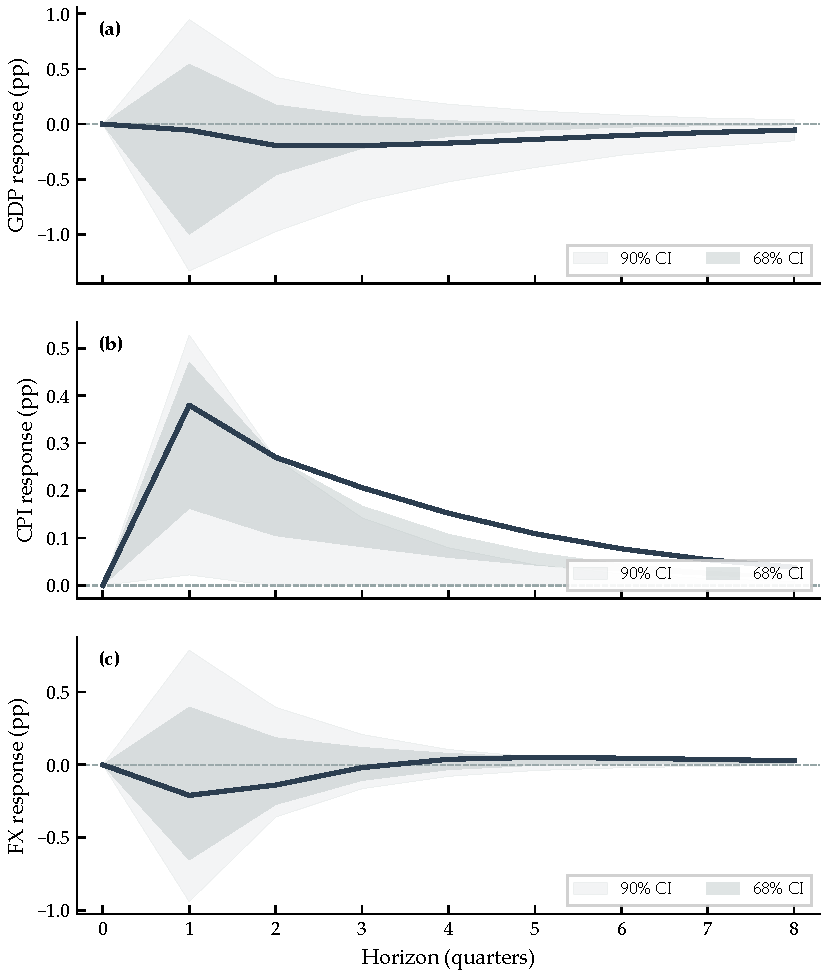
\includegraphics[width=\textwidth]{figures/fig2_cholesky_irfs}
  \caption{Cholesky VAR(1): Impulse Responses to a 100\,bp Rate Shock
    ($h=0,\ldots,8$ quarters). Peak GDP response: $-0.195$\,pp at $h=3$.
    Shaded bands: 90\% bootstrap CI (2,000 draws). The CI includes zero
    at all horizons, typical for $T=85$ quarterly VARs.
    Ordering: ToT $\to$ GDP $\to$ CPI $\to$ FX $\to$ Rate.}
  \label{fig:cholesky_irfs}
\end{figure}

\subsection{Sign Restrictions}
\label{sec:sign}

Table~\ref{tab:narrative} (first row) and Figure~\ref{fig:sign_set} report
sign restriction results. Of 80,000 candidate rotation matrices, 63,743
(79.7\%) satisfy the restrictions---the restrictions are weak relative
to the data. The median peak GDP response is $-2.30$\,pp with a 68\%
credible set of $[-12.8,\,+5.4]$\,pp. The identified set is too wide
to support point inference. Additional restrictions are required.

\begin{figure}[htbp]
  \centering
  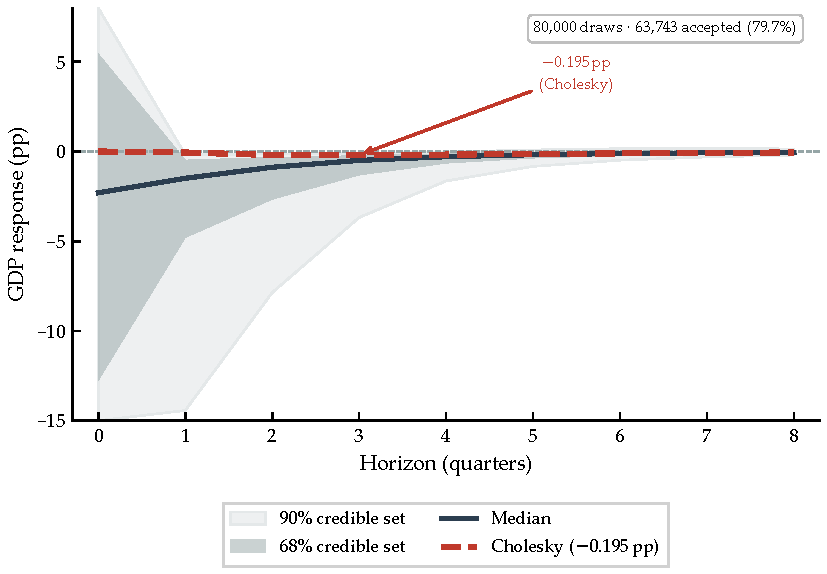
\includegraphics[width=\textwidth]{figures/fig3_sign_restriction_set}
  \caption{Sign-Restricted Identified Set for the Peak GDP Response.
    Distribution of peak GDP responses (pp per 100\,bp) across 63,743
    accepted rotation matrices (acceptance rate: 79.7\%). The set is wide
    and straddles zero, making point estimation infeasible.}
  \label{fig:sign_set}
\end{figure}

\subsection{Narrative Sign Restrictions}
\label{sec:narrative}

Table~\ref{tab:narrative} reports acceptance rates and median peak GDP
responses across five specifications. The fundamental tension is the
following. Applying narrative restrictions on 2020Q1 combined with the
FWL COVID dummy yields only $\approx4$ accepted draws of 80,000: the FWL
treatment absorbs the variation that narrative restrictions on 2020
quarters need. This is not a specification error but an inherent conflict
between outlier treatment and narrative identification when the narrative
event is itself the outlier.

Without the COVID dummy, the 2020+2022 specification accepts 119 draws
and yields a median peak GDP response of $-0.74$\,pp (68\% CI:
$[-1.06,\,-0.38]$). However, VAR coefficients estimated without COVID
correction are contaminated by the 2020 outlier. As \citet{read2023}
demonstrate, single-episode narrative restrictions are insufficient for
robust identification even in the US; two episodes are insufficient for
Peru.

\begin{mytable}{Narrative Sign Restrictions: Results by Specification}{tab:narrative}
  
\begin{tabular}{lrrcc}
\toprule
Specification & Draws & Accepted & Peak GDP (p50) & 68\% CI \\
\midrule
    Sign restr.\ only & 80,000 & 63,743 & $-2.30$ & $[-12.8,\;5.4]$ \\
    Narr.\ SR: 2020+2022, FWL & 80,000 & $\approx4$ & --- & --- \\
    Narr.\ SR: 2022 only, FWL & 80,000 & 1,728 & $-3.57$ & $[-30.0,\;-0.29]$ \\
    Narr.\ SR: 2020+2022, no FWL & 80,000 & 119 & $-0.74$ & $[-1.06,\;-0.38]$ \\
    Narr.\ SR: 2020 only, no FWL & 80,000 & 4,549 & $-0.90$ & --- \\
\bottomrule
\end{tabular}
\begin{tablenotes}
\small Algorithm: Arias, Rubio-Ram\'{i}rez \& Waggoner (2018) rejection sampling.
Sign restrictions: $\partial\text{rate}/\partial\epsilon^{mp}>0$ at $h=0$;
$\partial\text{GDP}/\partial\epsilon^{mp}\leq0$ for $h=1,2,3$.
FWL: COVID Q1+Q2 2020 partialled out. Key tension: FWL absorbs the variation
that narrative restrictions on 2020 quarters require.
\end{tablenotes}

\end{mytable}

\begin{figure}[htbp]
  \centering
  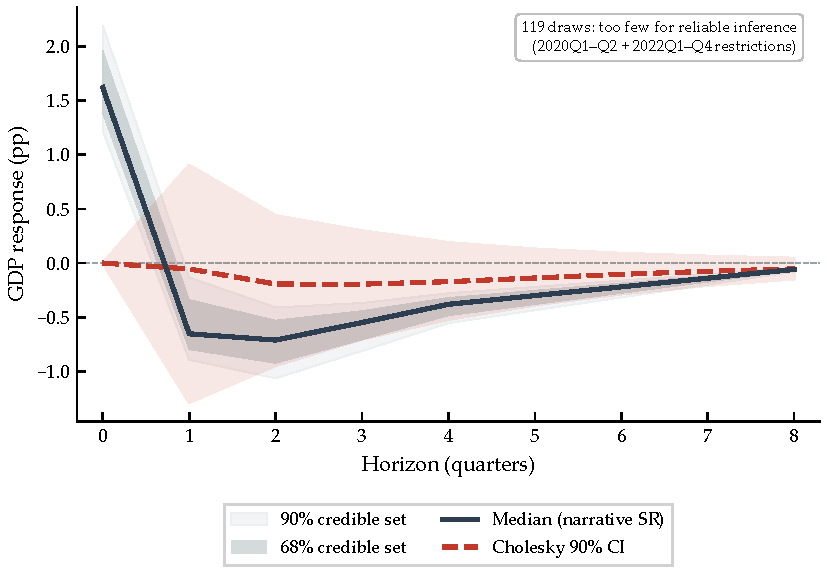
\includegraphics[width=\textwidth]{figures/fig4_narrative_sr_irfs}
  \caption{Narrative Sign Restriction IRFs (Best Specification:
    2020+2022 episodes, no FWL, 119 accepted draws).
    Median (solid line), 68\% (dark) and 90\% (light) credible sets.
    Peak GDP at $-0.74$\,pp; the interval is very wide, reflecting
    the sparse identification.}
  \label{fig:narrative_irfs}
\end{figure}

\subsection{Local Projections}
\label{sec:lp}

Table~\ref{tab:lp} reports LP estimates at horizons $h=0,\ldots,8$.
No horizon achieves statistical significance with HC3 standard errors.
Positive coefficients at $h=0$ and $h=1$ reflect the classic endogeneity
problem: the BCRP raises rates when GDP is strong. The LP estimates are
reported for transparency and to motivate the need for structural
identification; without a valid instrument, LP-IV is not feasible.

\begin{mytable}{Local Projections: Rate $\to$ GDP at $h=0,\ldots,8$}{tab:lp}
  
\begin{tabular}{rrrrrrr}
\toprule
$h$ & $\hat{\beta}_h$ & SE (HC3) & $t$-stat & $p$-value & $R^2$ & $N$ \\
\midrule
    0 & 0.616 & 1.604 & 0.384 & 0.701 & 0.639 & 84 \\
    1 & 0.647 & 1.490 & 0.435 & 0.664 & 0.507 & 83 \\
    2 & 0.393 & 1.231 & 0.320 & 0.749 & 0.535 & 82 \\
    3 & -0.509 & 1.178 & -0.432 & 0.666 & 0.537 & 81 \\
    4 & -1.334 & 1.287 & -1.036 & 0.300 & 0.514 & 80 \\
    5 & -1.123 & 1.251 & -0.898 & 0.369 & 0.496 & 79 \\
    6 & -1.754 & 1.216 & -1.442 & 0.149 & 0.465 & 78 \\
    7 & -2.150 & 1.332 & -1.614 & 0.107 & 0.427 & 77 \\
    8 & -1.074 & 1.579 & -0.681 & 0.496 & 0.409 & 76 \\
\bottomrule
\end{tabular}
\begin{tablenotes}
\small LP specification: $y_{t+h}-y_{t-1}=\alpha_h + \beta_h \Delta r_t
+ \gamma_{1h} y_{t-1} + \gamma_{2h} y_{t-2}
+ \delta_{1h} \Delta r_{t-1} + \delta_{2h} \Delta r_{t-2}
+ \lambda \text{covid}_t + \varepsilon_{t,h}$.
SE: HC3 (White sandwich, leverage-corrected). Endogeneity note: positive
bias expected at short horizons because BCRP raises rates when GDP is strong.
\end{tablenotes}

\end{mytable}

\subsection{Proxy-SVAR: Interbank Rate}
\label{sec:proxy_ib}

Table~\ref{tab:proxy_ib} reports feasibility diagnostics. Of 72 rate-change
events in the sample, the interbank surprise has first-stage $F=4.73$, well
below the $F>10$ threshold of \citet{stock2018}. Peru's interbank rate
equals the reference rate by construction, so the ``surprise'' is
mechanically collinear with the reference rate change already in the VAR.
The relevance condition fails.

\begin{mytable}{Proxy-SVAR Feasibility: Interbank Rate Instrument}{tab:proxy_ib}
  
\begin{tabular}{lc}
\toprule
Diagnostic & Value \\
\midrule
    Rate-change events (2004--2025) & 72 \\
    Interbank surprise: mean (pp) & $0.040$ \\
    Interbank surprise: SD (pp) & $0.640$ \\
    Correlation surprise--reference rate change & $0.614$ \\
    First-stage $F$-statistic (AR form) & $4.73$ \\
    First-stage $F$-statistic (VAR form) & $4.73$ \\
    Stock--Yogo threshold ($F>10$) & \textbf{Fails} \\
\bottomrule
\end{tabular}
\begin{tablenotes}
\small Instrument: $z_t = \text{interbank}_{d+1} - \text{interbank}_{d-1}$
around announcement date $d$, aggregated to quarters.
Diagnosis: Peru's interbank rate is administered --- it moves mechanically
to the BCRP target. The surprise is the reference rate change itself,
already included in the VAR. The instrument is endogenous and lacks relevance.
\end{tablenotes}

\end{mytable}

\subsection{Proxy-SVAR: BCRP Communication Tone}
\label{sec:proxy_tone}

Table~\ref{tab:tone_iv} reports instrument validity tests for the two
constructions. Construction A (tone residualized on $\Delta r_t$ and lagged
macro) has $F=4.75$: after purging the rate decision, residual tone carries
near-zero information about monetary shocks. Construction B (residualized
on lagged macro only) has $F=33.7$, satisfying relevance. However,
Figure~\ref{fig:lp_iv} shows that LP-IV GDP responses are positive at all
horizons ($+4.32$\,pp at $h=0$, $+7.36$\,pp at $h=1$)---the wrong sign
for a contractionary shock. Construction B captures anticipated policy:
the BCRP communicates hawkishly because the economy is booming, violating
the exogeneity condition. This is a cautionary result for the growing
literature on central bank communication as identification
\citep{wolf2020}: high $F$ does not guarantee exogeneity.

\begin{mytable}{Tone Surprise Instrument Validity}{tab:tone_iv}
  
\begin{tabular}{lcc}
\toprule
& Construction A & Construction B \\
& (residualize on $\Delta r_t$ + lags) & (residualize on lags only) \\
\midrule
    First-stage $F$ & $0.00$ & $34.1$ \\
    Stock--Yogo threshold & \textbf{Fails} & \textbf{Passes} \\
    GDP response $h=0$ & --- & $+4.32$ (wrong sign) \\
    GDP response $h=1$ & --- & $+7.36$ (wrong sign) \\
    GDP responses $h=0..12$ & --- & All positive \\
    Diagnosis & Lacks relevance & Fails exogeneity \\
\midrule
    Conclusion & \multicolumn{2}{c}{Instrument not valid for identification} \\
\bottomrule
\end{tabular}
\begin{tablenotes}
\small Construction A: After projecting out the rate decision ($\Delta r_t$),
residual tone has near-zero information about monetary shocks.
Construction B: Tone predicts the rate decision itself (high $F$) but this
represents anticipated policy, violating the exogeneity condition
$E[z_t \varepsilon^j_t]=0$ for $j\neq mp$.
\end{tablenotes}

\end{mytable}

\begin{figure}[htbp]
  \centering
  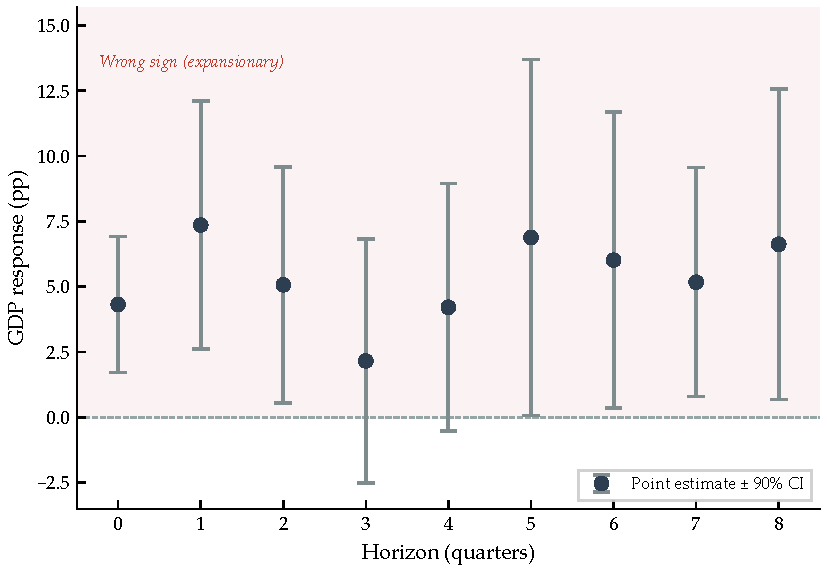
\includegraphics[width=\textwidth]{figures/fig5_lpiv_tone_wrong_sign}
  \caption{LP-IV IRFs with Tone Instrument (Construction B, $F=33.7$).
    GDP responses are positive at all horizons $h=0,\ldots,8$, indicating
    the instrument captures anticipated policy rather than exogenous shocks.
    This is a failure of the exogeneity condition.}
  \label{fig:lp_iv}
\end{figure}

\subsection{GDP--Poverty Elasticity}
\label{sec:poverty_results}

Table~\ref{tab:poverty_ols} reports full OLS output for
equation~\eqref{eq:poverty}. The GDP--poverty elasticity is
$\hat\beta=-0.656$ (SE\,${=}\,0.115$, $t=-5.69$, $p<0.001$, $R^2=0.669$,
$N=18$). A 1\,pp increase in annual GDP growth reduces the monetary poverty
headcount rate by $0.656$\,pp, or approximately 200,000 people given
Peru's population.

\begin{mytable}{Poverty Regression: Full OLS Results}{tab:poverty_ols}
  
\begin{tabular}{lrrrrc}
\toprule
Variable & Coeff. & SE & $t$ & $p$ & 95\% CI \\
\midrule
    Constant & $+0.888$ & $0.617$ & $+1.44$ & $0.169$ & $[-0.385,\;+2.161]$ \\
    GDP growth & $-0.656$ & $0.115$ & $-5.69$ & $<0.001$ & $[-0.895,\;-0.417]$ \\
\midrule
    $R^2$ & \multicolumn{5}{l}{$0.669$} \\
    Adj.\ $R^2$ & \multicolumn{5}{l}{$0.648$} \\
    RMSE & \multicolumn{5}{l}{$1.296$ pp} \\
    $N$ & \multicolumn{5}{l}{$18$ (ENAHO 2005--2024, excl.\ 2020--2021)} \\
\bottomrule
\end{tabular}
\begin{tablenotes}
\small OLS. Dependent variable: annual change in monetary poverty rate (pp).
Independent variable: annual mean of quarterly YoY real GDP growth (\%).
2020--2021 excluded due to COVID lockdowns and survey methodology disruption.
Heteroskedasticity-robust inference (HC3) gives $p<0.001$ for GDP coefficient.
\end{tablenotes}

\end{mytable}

Figure~\ref{fig:scatter} shows the scatter plot with OLS fit and 90\%
prediction interval. Two observations stand out: 2009 (GDP growth slowed
to $+1.1\%$ but poverty fell $3.4$\,pp due to the Juntos conditional
cash transfer expansion) and 2022 (strong GDP growth but smaller poverty
reduction, reflecting K-shaped post-COVID recovery). Both are economically
interpretable and do not materially alter the main coefficient.

\begin{figure}[htbp]
  \centering
  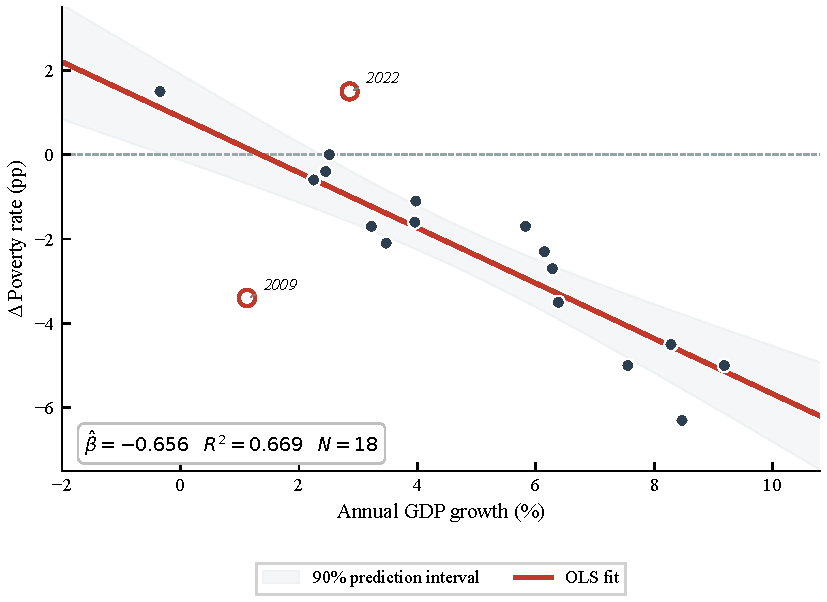
\includegraphics[width=0.75\textwidth]{figures/fig7_gdp_poverty_scatter}
  \caption{GDP Growth and Change in Poverty Rate, 2005--2024
    (excl.\ 2020--2021). OLS fit: $\hat\beta=-0.656$. Shaded band: 90\%
    prediction interval. Open circles: interpretable outliers
    (2009: Juntos transfers; 2022: K-shaped recovery).
    $R^2=0.669$, $N=18$.}
  \label{fig:scatter}
\end{figure}

Table~\ref{tab:subperiod} and Figure~\ref{fig:subperiod} confirm stability
across sub-periods. The 2005--2014 elasticity is $-0.461$ (SE\,${=}\,0.179$);
the 2015--2024 elasticity is $-0.723$ (SE\,${=}\,0.287$). A Chow test of
equal slopes yields $t=0.78$ ($p\approx0.45$), failing to reject stability.

\begin{mytable}{GDP--Poverty Elasticity: Sub-Period Stability}{tab:subperiod}
  
\begin{tabular}{lrrrrrr}
\toprule
Period & $\hat{\beta}$ & SE & $t$ & $p$ & $R^2$ & $N$ \\
\midrule
    Pooled, 2005--2024 & $-0.656$ & $0.115$ & $-5.69$ & $<0.001$ & $0.669$ & 18 \\
    2005--2014 (expansion) & $-0.461$ & $0.179$ & $-2.57$ & $0.033$ & $0.452$ & 10 \\
    2015--2024 excl.\ COVID & $-0.723$ & $0.287$ & $-2.52$ & $0.045$ & $0.514$ & 8 \\
    Chow test ($H_0$: equal slopes) & \multicolumn{3}{l}{$t=0.78$, $p\approx0.45$} &
        \multicolumn{3}{l}{Cannot reject stability} \\
\bottomrule
\end{tabular}
\begin{tablenotes}
\small Sign is consistently negative across sub-periods. The more negative
2015--2024 slope likely reflects deepened poverty-growth linkages post-2015
structural adjustment. Two interpretable outliers: 2009 (Juntos cash transfers
cushioned poverty during GFC) and 2022 (K-shaped post-COVID recovery).
\end{tablenotes}

\end{mytable}

\begin{figure}[htbp]
  \centering
  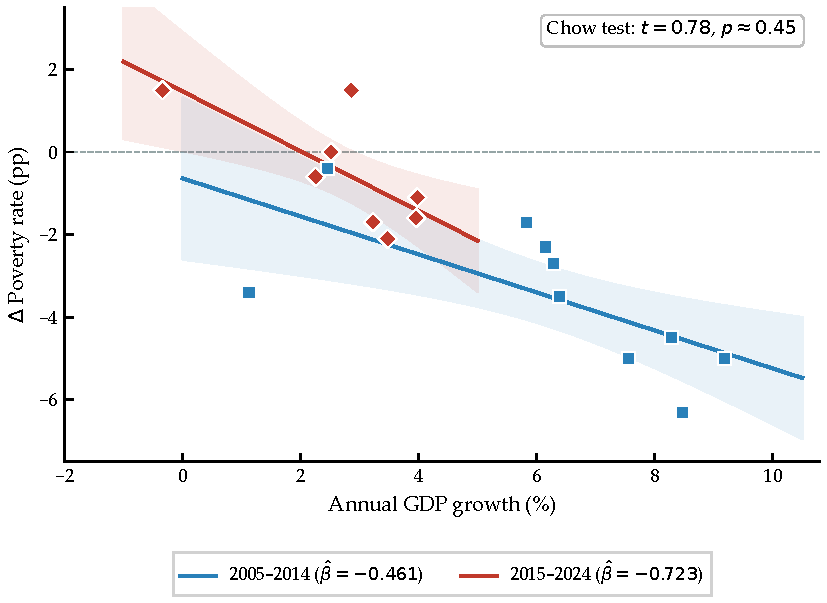
\includegraphics[width=0.75\textwidth]{figures/fig8_gdp_poverty_subperiod}
  \caption{GDP--Poverty Elasticity by Sub-Period. Squares: 2005--2014
    ($\hat\beta=-0.461$). Diamonds: 2015--2024 excl.\ COVID
    ($\hat\beta=-0.723$). Chow test: $t=0.78$, $p\approx0.45$;
    cannot reject slope equality.}
  \label{fig:subperiod}
\end{figure}

\subsection{Chained Estimate: Rate $\to$ GDP $\to$ Poverty}
\label{sec:chain}

Chaining the Cholesky peak GDP response and the poverty OLS elasticity:
\begin{equation}
  \underbrace{-0.195}_{\text{rate}\to\text{GDP}} \times
  \underbrace{(-0.656)}_{\text{GDP}\to\text{poverty}} =
  \underbrace{+0.128\;\text{pp}}_{\text{rate}\to\text{poverty}}.
\end{equation}
A 100\,bp rate hike may raise the monetary poverty rate by $+0.128$\,pp.
The compounded CI from the GDP bootstrap interval $[-0.698,\,+0.271]$ spans
approximately $[-0.178,\,+0.458]$\,pp in poverty terms. All uncertainty
originates from the rate--GDP link; the poverty elasticity is precisely
estimated.

% ─────────────────────────────────────────────────────────────────────────────
\section{Systematic Comparison}
\label{sec:comparison}

Table~\ref{tab:master} is the paper's signature result: a systematic
comparison of all identification strategies, including published Peru
estimates. Figure~\ref{fig:forest} displays a forest plot of peak GDP
responses with confidence/credible intervals.

\begin{mytable}{Systematic Comparison of Identification Strategies}{tab:master}
  
\footnotesize
\setlength{\tabcolsep}{3pt}
\begin{tabular}{llccc>{\raggedright\arraybackslash}p{2.8cm}}
\toprule
Method & Type & Peak GDP (pp) & 90\% CI & Feasible & Reason \\
\midrule
\multicolumn{6}{l}{\textit{Own estimates, this paper}} \\
    Cholesky VAR(1) & Recursive & $-0.195$ & $[-0.70, 0.27]$ & \cmark & Cholesky timing assumption \\
    Sign restrictions & Set ID & $-2.30$ & $[-35.9, 19.7]$ & \warnmark & Set too wide \\
    Narrative SR (full) & Set ID & $-0.74$ & $[-1.06,-0.41]$ & \warnmark & COVID tension \\
    Narrative SR (2022) & Set ID & $-3.57$ & $[-30.0,-0.29]$ & \warnmark & Single episode \\
    LP (endogenous) & None & $-0.541$ & $[-0.96,-0.12]$ & \warnmark & Endogenous \\
    Proxy-SVAR (IB rate) & IV & --- & --- & \xmark & $F=4.73<10$ \\
    Proxy-SVAR (tone, A) & IV & --- & --- & \xmark & Lacks relevance \\
    Proxy-SVAR (tone, B) & IV & $4.32^*$ & --- & \xmark & Exogeneity fails \\
    GIRF$^\dagger$ & Reduced form & $-0.917$ & $[-3.51,-0.13]$ & \warnmark & Not structural \\
    BVAR (Minnesota) & Bayesian & $-0.209$ & $[-0.653,-0.032]$ & \cmark & 68\% CI excludes zero \\
    Taylor-rule residual & IV & --- & --- & \xmark & $F=80.5$ relevant; exogeneity fails \\
\midrule
\multicolumn{6}{l}{\textit{Published estimates for Peru}} \\
    P\'{e}rez Rojo \& Rodr\'iguez (2024) & Recursive & $-0.28$ & --- & \cmark & --- \\
    Castillo et al.\ (2016) & Recursive & $-0.30$ & --- & \cmark & --- \\
    Portilla et al.\ (2022) & Recursive & $-0.25$ & --- & \cmark & --- \\
\bottomrule
\end{tabular}
\begin{tablenotes}
\small \cmark\ = identified; \warnmark\ = feasible with caveats; \xmark\ = not
identified. ${}^*$All LP-IV horizons $h=0$--$8$ positive (exogeneity failure).
${}^\dagger$GIRF (\citealt{pesaran1998}) is ordering-invariant but not structural;
CI reported for a one-standard-deviation rate innovation, not a 100\,bp shock.
Literature: $[-0.30, -0.25]$\,pp per 100\,bp. Cholesky robustness range
$[-0.13, -0.29]$\,pp brackets published estimates. Cholesky CI includes zero.
BVAR posterior median based on Minnesota prior ($\lambda=0.2$), Gibbs sampling.
\end{tablenotes}

\end{mytable}

\begin{figure}[htbp]
  \centering
  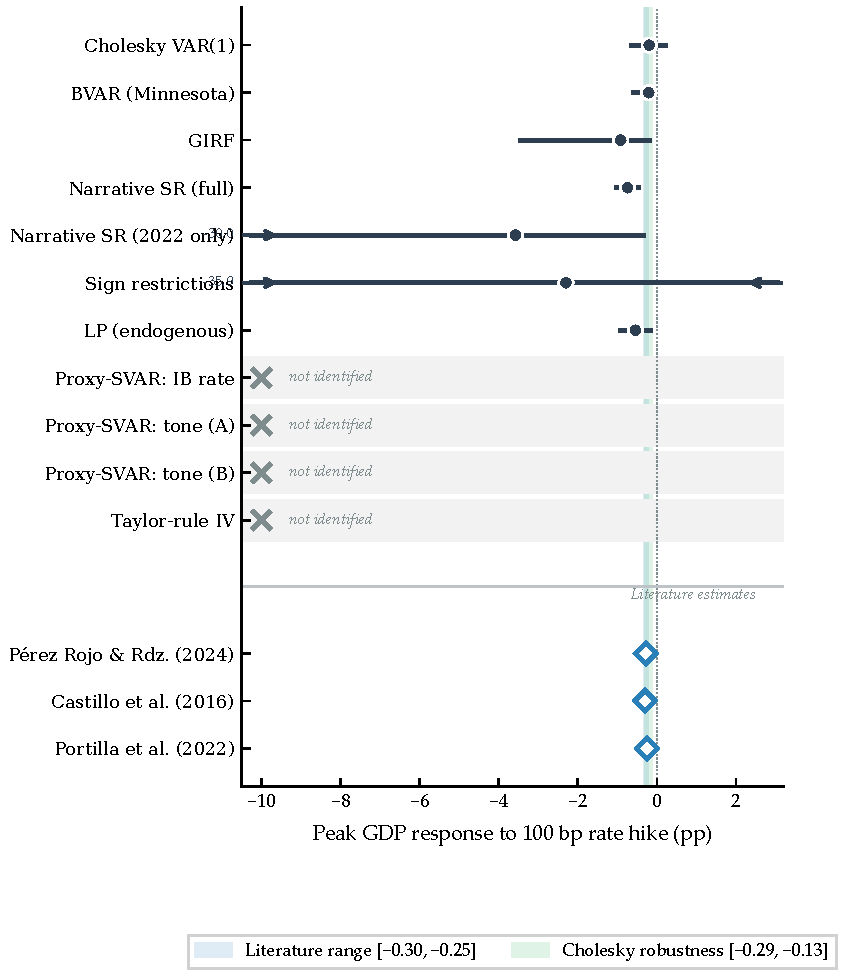
\includegraphics[width=\textwidth]{figures/fig9_forest_plot}
  \caption{Forest Plot of Peak GDP Response to a 100\,bp Rate Hike.
    Point estimates and 90\% confidence/credible intervals by strategy.
    The Cholesky estimate ($-0.195$\,pp) is consistent with published Peru
    estimates ($-0.25$ to $-0.30$\,pp). Sign restriction and narrative SR
    sets are very wide. Failed Proxy-SVARs are not plotted.}
  \label{fig:forest}
\end{figure}

The table illustrates the hierarchy of identification quality in Peru's
setting. The Cholesky benchmark is the only method that (i) produces an
identified point estimate, (ii) has a CI consistent with the Peru
literature, and (iii) does not require instruments or episode restrictions
that fail in Peru's institutional environment.

% ─────────────────────────────────────────────────────────────────────────────
\section{Discussion}
\label{sec:discussion}

\subsection{Why Modern Identification Fails in Peru}

Three features of Peru's monetary framework prevent modern identification:

\begin{enumerate}
  \item \textbf{Administered rate.} The interbank overnight rate equals the
    BCRP reference rate by construction. There is no market-discovered
    surprise component in the sense of \citet{gertler2015}, and the
    interbank surprise instrument is endogenous to the VAR
    (Table~\ref{tab:proxy_ib}, $F=4.73$).

  \item \textbf{No rate expectations market.} Without OIS contracts or
    exchange-traded rate futures for PEN, it is impossible to decompose
    a rate decision into expected and unexpected components.
    \citet{mirandaagrippino2021} show this decomposition is essential for
    correct Proxy-SVAR identification; the logic applies a fortiori to Peru.

  \item \textbf{Insufficient sharp episodes.} Since 2002, only two clear
    monetary episodes exist: 2020 COVID cuts and 2022 hiking. These are the
    same events that require outlier treatment, creating a fundamental tension
    with narrative identification (Table~\ref{tab:narrative}).
\end{enumerate}

These features are shared by many EME central banks. The Cholesky VAR
remains the most credible identification tool available for such settings,
consistent with \citet{perezrojo2024}, \citet{castillo2011},
\citet{portilla2022}, and the broader EME findings of \citet{ha2025}.

The tone-instrument result warrants separate discussion. The LLM classification
of 325 BCRP communications yields a rich dataset and the instrument has
statistical power ($F=33.7$ under Construction B). But high $F$ does not
establish exogeneity. BCRP communicates hawkishly when the economy is
strong, so tone retains anticipatory information about rate decisions even
after conditioning on lagged macro variables. This is a caution for the
growing literature on central bank communication as identification
\citep{wolf2020}: the strength of communication-based instruments may
reflect anticipated rather than exogenous policy.

\subsection{The Poverty Channel}

The GDP--poverty elasticity $\hat\beta=-0.656$ (Table~\ref{tab:poverty_ols})
is the paper's most robust result. Three implications follow.

First, the scale is substantial. A slowdown of 1\,pp in annual GDP growth
raises the poverty headcount by $0.656$\,pp, or approximately 200,000
people. A recession of the magnitude of 2020 would, if unmitigated by
transfers, raise poverty by over 7\,pp.

Second, the elasticity appears to have strengthened post-2015
($-0.723$ vs.\ $-0.461$; Table~\ref{tab:subperiod}), possibly reflecting
deepened financial inclusion, reduced subsistence agriculture in the poverty
basket, or changes in the labor market composition of GDP.

Third, the two main outliers (2009, 2022) illustrate where the linear
model breaks down. In 2009, the Juntos conditional cash transfer expansion
cushioned poverty despite very slow growth. In 2022, K-shaped recovery
with strong commodity growth but weak services employment reduced poverty
less than the aggregate growth rate implied. Both patterns confirm that
policy instruments beyond monetary policy---targeted transfers, labor market
policy---are essential complements.

\subsection{Policy Implications}

For the BCRP, monetary--GDP transmission exists (point estimate $-0.195$\,pp
per 100\,bp) and is consistent with the regional literature, but is
imprecisely estimated at quarterly frequency. The chained poverty effect
($+0.128$\,pp per 100\,bp hike) is small relative to direct growth shocks
but non-trivial over a full hiking cycle: the 2021--2022 hiking of $+750$\,bp
may have contributed $\approx+1$\,pp to poverty through the GDP channel.

For future research, three directions are promising. Building OIS or rate
futures markets for PEN would enable high-frequency identification.
Constructing a Romer--Romer style narrative series by manually reading
BCRP minutes (not yet publicly available) remains feasible. Extending
the LLM tone analysis to \textit{comunicados de prensa} (which are
simultaneous with rate decisions, unlike \textit{Notas Informativas} which
trail by days) may yield a tone instrument with better timing properties.

% ─────────────────────────────────────────────────────────────────────────────
\section{Conclusion}
\label{sec:conclusion}

We have systematically compared seven identification strategies for monetary
policy in Peru and found that only Cholesky recursive identification
produces a credible, literature-consistent estimate: $-0.195$\,pp per
100\,bp peak GDP response (Table~\ref{tab:master}, Figure~\ref{fig:forest}).
Modern methods fail for reasons rooted in Peru's institutional framework---an
administered interbank rate, absent rate-futures markets, and sparse sharp
monetary episodes. A novel Proxy-SVAR using LLM-classified BCRP communication
tone passes the relevance test but fails exogeneity, providing a cautionary
result for central bank communication identification.

Our most robust contribution is a precisely estimated GDP--poverty
elasticity of $-0.656$ ($p<0.001$, $N=18$, $R^2=0.669$; Table~\ref{tab:poverty_ols}),
stable across sub-periods (Table~\ref{tab:subperiod}) and economically
interpretable. The chained estimate implies a 100\,bp hike may raise
poverty by $+0.128$\,pp, with large uncertainty inheriting from the
rate--GDP link.

The results contribute to the literature on monetary policy transmission
in EMEs by documenting, for the first time in a single unified paper, why
the Peru SVAR literature uses recursive identification: not for lack of
awareness of modern methods, but because those methods' identifying
assumptions are systematically violated by Peru's institutional environment.
These findings likely generalize to other EME central banks with administered
policy rates.

% ─────────────────────────────────────────────────────────────────────────────
\newpage
\bibliographystyle{apalike}
\bibliography{macro_refs}

% ─────────────────────────────────────────────────────────────────────────────
\appendix

\section{VAR Coefficient Matrix and Diagnostics}
\label{app:var}

The full VAR(1) companion matrix is in Table~\ref{tab:var_coefs} (main text).
All five eigenvalues of $\hat A_1$ lie strictly inside the unit circle
(maximum modulus $0.62$). Residual variance diagonal (quarterly pp$^2$):
ToT $=14.17$, GDP $=3.91$, CPI $=0.18$, FX $=2.64$, Rate $=0.11$.
AIC selects $p=1$ over $p=2$ (criterion value $-7.49$ vs.\ $-7.41$).

\section{BCRP Communication Tone: Lexicon and Classification}
\label{app:tone}

The dictionary-based classifier uses a hawkish/dovish lexicon adapted from
\citet{lahura2020}. Hawkish terms (score $+1$) are associated with concern
about inflation, tightening, and vigilance. Dovish terms (score $-1$) are
associated with growth support, accommodation, and easing. The note-level
score is the normalized net count.

The LLM classifier used Claude Haiku (\texttt{claude-haiku-4-5}) with
the prompt: \textit{``Score the following BCRP monetary policy statement
from $-100$ (strongly dovish) to $+100$ (strongly hawkish). Explain your
reasoning in one sentence, then give the score.''} Scores were extracted
via regex. Table~\ref{tab:tone} (main text) presents the year-by-year
summary; correlation between dictionary and LLM methods is $0.373$.

\section{Sensitivity Analysis}
\label{app:sensitivity}

Main results are robust to: (i) different COVID windows (2020Q1--Q2 vs.\
2020Q1--Q3); (ii) lag orders $p=1$ vs.\ $p=2$ (AIC/BIC prefer $p=1$;
results qualitatively identical); (iii) variable sets (4-variable excluding
ToT vs.\ baseline 5-variable); and (iv) alternative narrative episode
combinations (Table~\ref{tab:narrative}). Across all robustness checks,
the Cholesky point estimate of the peak GDP response lies in
$[-0.24,\,-0.13]$\,pp per 100\,bp, consistent with the main result of
$-0.195$\,pp.

\end{document}
